\chapter{Results} \label{chap:results}

\section*{}

% Dependendo do volume, a avaliação do trabalho pode ser incluída no
% capítulo anterior ou pode constituir um capítulo separado.

This chapter provides the results obtained during this dissertation
and the analysis of these.

Section~\ref{sec:results:perf} reports several performance improvements
to the implemented \evm{} method and the developed algorithm to estimate
a person's heart rate.

Section~\ref{sec:results:heart} compares the measurements from the implemented
Android application, Pulse, to a sphygmomanometer, and also, to another
Android application by ViTrox that estimates a person's heart rate using
a different method.

\section{Performance} \label{sec:results:perf}

Smartphone devices have a low computational power and this was one of the
main difficulties. The first implementations of the application were not
fast enough and the implemented Android application running on a
\emph{HUAWEI MediaPad} tablet with the Android version 4.0.3 was only capturing
around 2 frames per second.

In order to improve the algorithm and application performance, metrics were
obtained using the \emph{High performance C++ Profiler}~\cite{Andrew2013High}.
This profiler was chosen because of its performance claim and easy integration
in the project.

The machine specifications on which all metrics were obtained are:

\begin{description}
  \item[Machine] MacBook Pro, 15-inch, Late 2008
  \item[Processor] 2.53 GHz Inter Core 2 Duo
  \item[Memory] 4 GB 1067 MHz DDR3
  \item[Operating System] OS X Mountain Lion
\end{description}

The input video used was the video \emph{face} found at~\cite{Wu2013Eulerian}.

On appendix~\ref{appx:perf} various tables can be found representing
several performance boosts accomplished. The unit used by the
\emph{High performance C++ Profiler} is the number of CPU cycles spent by
that operation, obtained by using the instruction
\texttt{rdtsc}~\cite{Andrew2013High}.

The main functions that needed to be optimized and analyzed are:

\begin{itemize}
  \item \texttt{Pulse::onFrame}, which is the function that detects a
        person face and estimates the heart rate for each face detected;
  \item \texttt{EvmGdownIIR::onFrame}, which is the function that
        implements the \evm{} method.
\end{itemize}

Table~\ref{tab:profile:initial} shows that these functions were spending
a big percentage of the CPU cycles, with the \texttt{Pulse} function
taking 51\% and the \evm{} method occupying 28\%.

\begin{table}[t]
  \centering
  \begin{tabular}{lrrr}
    \hline
    Operation & Calls & MCycles & Avg \\
    \hline
    Pulse::onFrame        & 301 & 15630.5432 ( 51\%) & 51.9287 \\
    EvmGdownIIR::onFrame  & 301 &  8507.6548 ( 28\%) & 28.2646 \\
    \hline
  \end{tabular}
  \caption{
    Performance metrics obtained form the initial implementation of the C/C++
    version of the desktop application. Excerpt from~\ref{pdf:profile:1}.
  }
  \label{tab:profile:initial}
\end{table}

The operations taking more CPU cycles were easily identified by the
second table on~\ref{pdf:profile:1}, also represented on
table~\ref{tab:profile:top}. These operations are:

\begin{itemize}
  \item OpenCV HighGUI module functions: \emph{wait key}, \emph{imshow},
        \emph{capture};
  \item resize operations: \emph{pyrUp}, \emph{pyrDown}, \emph{resize face box},
        and \emph{resize and draw face box back to frame};
  \item conversion operations: \emph{convert to 8 bit}, \emph{convert to float};
  \item matrix operations: \emph{add back to original frame};
  \item \emph{detect faces} operation, is the OpenCV object detector, details on
        section~\ref{sec:impl:face};
  \item \emph{detrend} operation, is the detrending method explained on
        section~\ref{sec:sota:post:detrend};
\end{itemize}

\begin{table}
  \centering
  \begin{tabular}{lrrr}
    \hline
    Operation & Calls & Self MCycles & Self Avg \\
    \hline
    wait key                                & 301 & 9892.1852 (32\%) & 32.8644 \\
    pyrUp                                   & 300 & 3472.5267 (11\%) & 11.5751 \\
    detect faces                            & 301 & 2941.3343 (10\%) & 9.7719  \\
    imshow                                  & 301 & 2555.0751 ( 8\%) & 8.4886  \\
    capture                                 & 302 & 2268.6110 ( 7\%) & 7.5120  \\
    pyrDown                                 & 301 & 1988.4146 ( 7\%) & 6.6060  \\
    convert to 8 bit                        & 300 & 1603.1581 ( 5\%) & 5.3439  \\
    detrend                                 & 301 & 1538.8180 ( 5\%) & 5.1124  \\
    resize face box                         & 301 & 1270.4278 ( 4\%) & 4.2207  \\
    resize and draw face box back to frame  & 301 & 1214.4998 ( 4\%) & 4.0349  \\
    add back to original frame              & 300 & 811.3654  ( 3\%) & 2.7046  \\
    convert to float                        & 301 & 604.0527  ( 2\%) & 2.0068  \\
    \hline
  \end{tabular}
  \caption{
    Operations taking more CPU cycles on the initial implementation of
    the C/C++ version of the desktop application when performance
    profiling was added. Excerpt from~\ref{pdf:profile:1}.
  }
  \label{tab:profile:top}
\end{table}

The first performance boost was achieved by replacing the resize operations
by faster resize methods. All together the resize operations were spending
26\% of the CPU cycles as shown by table~\ref{tab:profile:top}.
The optimizations for the operations \emph{pyrUp} and
\emph{pyrDown} are detailed on section~\ref{sec:impl:evm:final}.
The rest of the resize operations were changed to use the OpenCV
nearest neighbor interpolation method since the difference of size was small.
These optimizations reduced the total percentage of the CPU cycles
to 7\% as shown on table~\ref{tab:profile:resize}.

\begin{table}
  \centering
  \begin{tabular}{lrrr}
    \hline
    Operation & Calls & Self MCycles & Self Avg \\
    \hline
    pyrUp                                   & 300 & 583.2825 (2\%) & 1.9443 \\
    pyrDown                                 & 301 & 510.0373 (2\%) & 1.6945 \\
    resize and draw face box back to frame  & 301 & 430.7046 (2\%) & 1.4309 \\
    resize face box                         & 301 & 307.4483 (1\%) & 1.0214 \\
    \hline
  \end{tabular}
  \caption{
    Performance improvement on resize operations by using faster interpolations
    methods. Excerpt from~\ref{pdf:profile:2}.
  }
  \label{tab:profile:resize}
\end{table}

The second performance boost was accomplished by reducing the number of
executions of the OpenCV object detector. This operation was occupying
around 10\% of the CPU cycles as shown by table~\ref{tab:profile:top}.
By executing the face detection operation once every 10 frames its number
of CPU cycles was greatly reduced to 1\% as shown on
table~\ref{tab:profile:face}.

\begin{table}
  \centering
  \begin{tabular}{lrrr}
    \hline
    Operation & Calls & Self MCycles & Self Avg \\
    \hline
    detect faces &  30 & 288.2041 (1\%) & 9.6068 \\
    \hline
  \end{tabular}
  \caption{
    Performance improvement on face detection by reducing the number of times
    the OpenCV object detector was executed. Excerpt from~\ref{pdf:profile:3}.
  }
  \label{tab:profile:face}
\end{table}

A last performance boost applied to the implemented algorithm was the removal of
the resize operations \emph{resize face box} and
\emph{resize and draw face box back to frame} by modifying the \evm{} method
implemented which removed the requirement of the input image to be always of the
same size.

The result of these performance improvements are shown on
table~\ref{tab:profile:final}. With the \texttt{Pulse} function spending
only 14\% of the CPU cycles and a performance improvement of 37\%,
and the \evm{} method occupying 6\% of the CPU cycles and a performance
improvement of 22\%.

\begin{table}
  \centering
  \begin{tabular}{lrrr}
    \hline
    Operation & Calls & MCycles & Avg \\
    \hline
    Pulse::onFrame       & 300 & 4215.0788 ( 14\%) & 14.0503 \\
    EvmGdownIIR::onFrame & 287 & 1818.3953 (  6\%) &  6.3359 \\
    \hline
  \end{tabular}
  \caption{
    Final performance metrics of the main functions.
    Excerpt from~\ref{pdf:profile:4}.
  }
  \label{tab:profile:final}
\end{table}

This allowed for the implemented Android application to run at approximately
15 frames per second on the same Android device previously mentioned.

\section{Heart rate comparison} \label{sec:results:heart}

To validate the heart rate values obtained by the implemented Android
application a test was run and readings obtained to a total of 9 participants.
The procedure for the test was as follows:

\begin{enumerate}
  \item use the implemented Android application, named Pulse, to obtain an
        estimation of the person's heart rate, while at the same time
        obtain a reading from a sphygmomanometer, which also produces an
        average of the heart rate at the end, which would take
        approximately 30 seconds;
  \item then, in order to compare the results to another application,
        step one was repeated using the ViTrox application:
        \emph{What's My Heart Rate}~\cite{Vitrox2013};
  \item finally, each person was asked to do some physical exercise so
        their heart rate would increase, then step one was repeated.
\end{enumerate}

Tables~\ref{tab:heart} shows the measurements obtained by the above procedure.
In order to interpret the measurements, Bland-Altman
plots~\cite{Martin1986Statistical} were used.
The mean and standard deviation~(SD) of the differences, mean of the absolute
differences and 95\% limits of agreement ($\pm$ 1.96 SD) were calculated.

Comparing the Bland-Altman plots in figure~\ref{fig:plots:heart}, the ViTrox
application shows the best agreement against the sphygmomanometer,
figure~\ref{fig:plots:heart:vitrox:normal}; the mean bias was $1.33$ bpm
with 95\% limits of agreement $-3.56$ to $6.22$ bpm. In comparison,
the implemented application, Pulse, had a mean bias of $-12.00$ with
95\% limits of agreement $-33.13$ to $9.13$ bpm,
figure~\ref{fig:plots:heart:pulse:normal}, and after the physical exercise,
figure~\ref{fig:plots:heart:pulse:exercise}, the mean bias was $-25.89$
with 95\% limits of agreement $-51.28$ to $-0.49$ bpm.

The implemented algorithm has worse estimations with higher heart rates.
However, by picking only heart rates lower than 70 bpm according to the
sphygmomanometer, table~\ref{tab:heart:pulse:low} and
figure~\ref{fig:plots:heart:pulse:low}, the agreement between the
implemented application, Pulse, and the sphygmomanometer increases to
a mean bias of $-4.25$ with 95\% limits of agreement $-13.43$ to $4.93$ bpm.

It should be noted that the main goal of this dissertation was testing the
feasibility of implementing an \evm{}-based method on a mobile device with
the Android platform. The creation of an Android application to monitor
a person's heart rate was a simple example of the application of the
performance optimized \evm{} method developed.
Hence, the effort taken on the algorithm performance was higher than
the validation of the heart rate estimation algorithm.

% Bland-Altman values
%% pulse-normal
% mean             = -12.00
% mean + 1.96 * SD =   9.13
% mean - 1.96 * SD = -33.13
%% vitrox-normal
% mean             =   1.33
% mean + 1.96 * SD =   6.22
% mean - 1.96 * SD =  -3.56
%% pulse-after-exercise
% mean             = -25.89
% mean + 1.96 * SD =  -0.49
% mean - 1.96 * SD = -51.28
%% pulse-lower-than-70-bpm
% mean             =  -4.25
% mean + 1.96 * SD =   4.93
% mean - 1.96 * SD = -13.43

\begin{table}[p]
  \begin{subtable}{0.5\textwidth}
    \centering
    \begin{tabular}{crr}
      \hline
        Participant & \multilinecell{Pulse\\(bpm)} & \multilinecell{Sphy.\\(bpm)} \\
      \hline
        A & 55 & 57 \\
        B & 60 & 60 \\
        C & 57 & 76 \\
        D & 54 & 66 \\
        E & 47 & 75 \\
        F & 54 & 57 \\
        G & 55 & 84 \\
        H & 62 & 83 \\
        I & 56 & 59 \\
        I & 55 & 58 \\
      \hline
        Mean & 55.50 & 67.50 \\
        SD   &  3.98 & 10.97 \\
      \hline
    \end{tabular}
    \caption{
      Heart rate measurements obtained at the same time from the implemented
      Android application, Pulse, and the sphygmomanometer.
    }
    \label{tab:heart:pulse:normal}
  \end{subtable}
  ~
  \begin{subtable}{0.5\textwidth}
    \centering
    \begin{tabular}{crr}
      \hline
        Participant & \multilinecell{ViTrox\\(bpm)} & \multilinecell{Sphy.\\(bpm)} \\
      \hline
        A & 66 & 61 \\
        B & 61 & 57 \\
        C & 72 & 72 \\
        D & 65 & 63 \\
        E & 81 & 77 \\
        F & 55 & 56 \\
        G & 87 & 87 \\
        H & 79 & 82 \\
        I & 55 & 54 \\
      \hline
        Mean & 69.00 & 67.67 \\
        SD   & 11.50 & 12.19 \\
      \hline
    \end{tabular}
    \caption{
      Heart rate measurements obtained at the same time from the ViTrox
      Android application and the sphygmomanometer.
    }
    \label{tab:heart:vitrox:normal}
  \end{subtable}

  \begin{subtable}{0.5\textwidth}
    \centering
    \begin{tabular}{crr}
      \hline
        Participant & \multilinecell{Pulse\\(bpm)} & \multilinecell{Sphy.\\(bpm)} \\
      \hline
        A & 54 &  87 \\
        B & 66 &  65 \\
        C & 57 &  98 \\
        D & 48 &  71 \\
        E & 64 &  84 \\
        F & 51 &  63 \\
        G & 69 & 102 \\
        H & 66 & 105 \\
        I & 47 &  80 \\
      \hline
        Mean & 58.00 & 83.89\\
        SD   &  8.46 & 15.64 \\
      \hline
    \end{tabular}
    \caption{
      Heart rate measurements obtained at the same time from the implemented
      Android application, Pulse, and the sphygmomanometer, after physical
      exercise.
    }
    \label{tab:heart:pulse:exercise}
  \end{subtable}
  ~
  \begin{subtable}{0.5\textwidth}
    \centering
    \begin{tabular}{crr}
      \hline
        Participant & \multilinecell{Pulse\\(bpm)} & \multilinecell{Sphy.\\(bpm)} \\
      \hline
        A & 55 & 57 \\
        B & 60 & 60 \\
        B & 66 & 65 \\
        D & 54 & 66 \\
        F & 54 & 57 \\
        F & 51 & 63 \\
        I & 56 & 59 \\
        I & 55 & 58 \\
      \hline
        Mean & 56.38 & 60.63 \\
        SD   &  4.63 &  3.58 \\
      \hline
    \end{tabular}
    \caption{
      Selection of heart rate measurements obtained from the Pulse application
      with an heart rate of 70 bpm or lower according to the sphygmomanometer.
    }
    \label{tab:heart:pulse:low}
  \end{subtable}

  \caption{
    Heart rate measurements obtained following the procedure described
    from a sphygmomanometer and an Android application:
    either Pulse, (a), (c), (d), which is the developed application,
    or the ViTrox application, (b).
  }
  \label{tab:heart}
\end{table}

\begin{figure}[p]
  \begin{subfigure}{0.5\textwidth}
    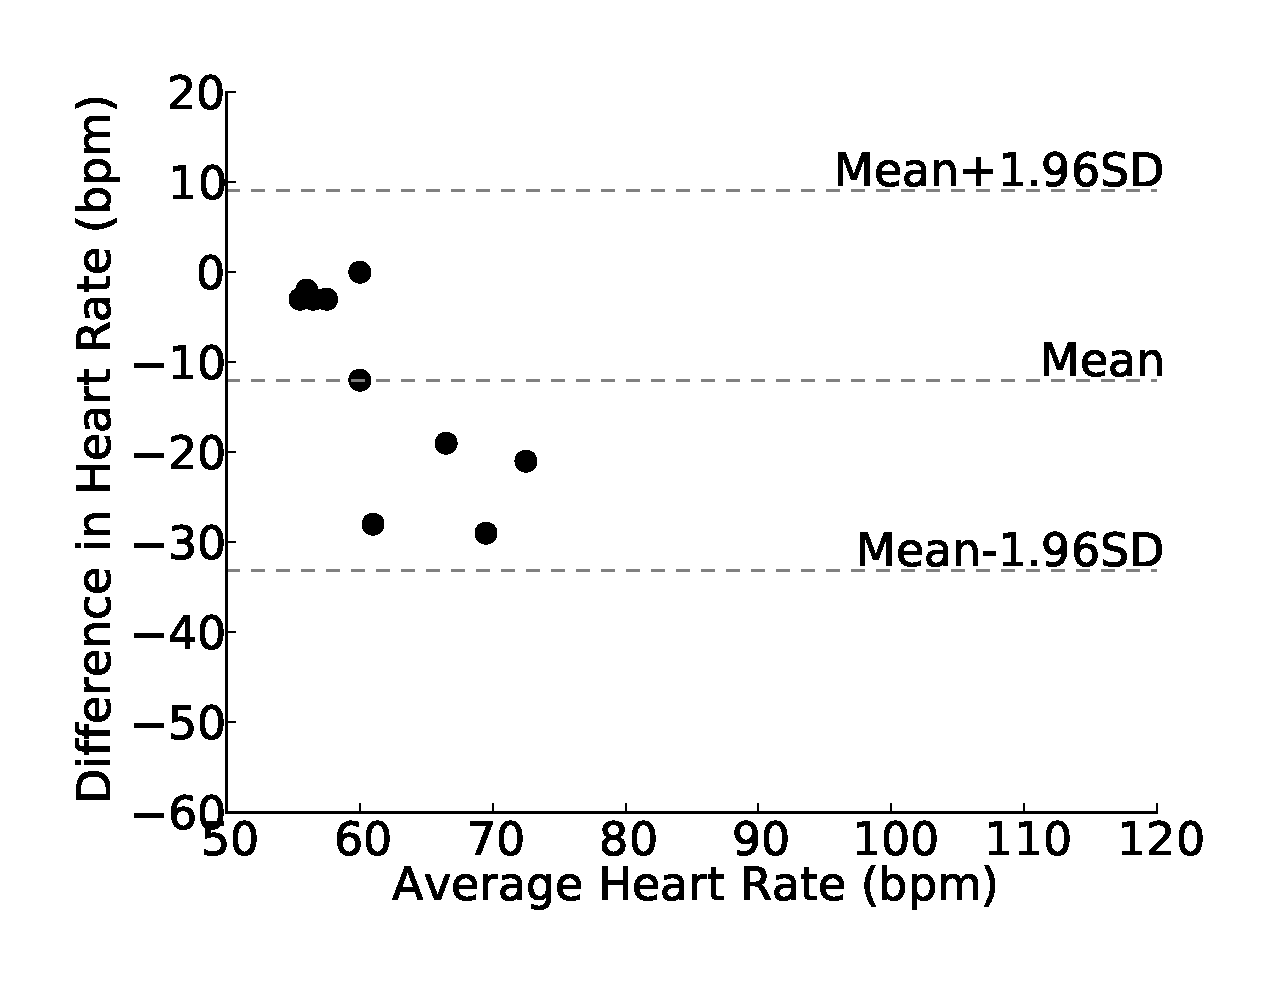
\includegraphics[width=\textwidth]{plots/pulse-normal}
    \caption{Pulse and sphygmomanometer.}
    \label{fig:plots:heart:pulse:normal}
  \end{subfigure}
  ~
  \begin{subfigure}{0.5\textwidth}
    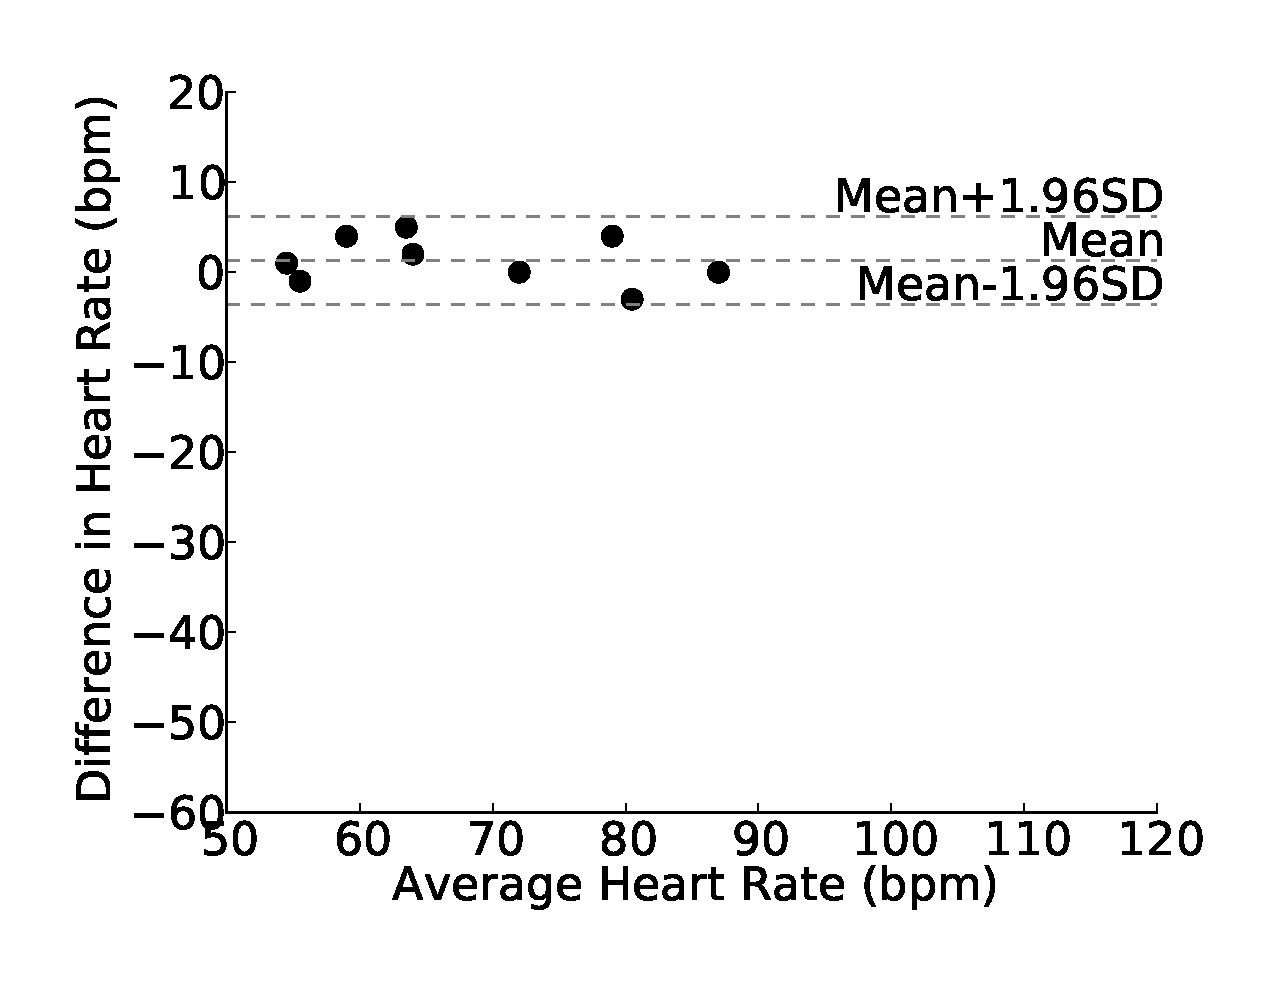
\includegraphics[width=\textwidth]{plots/vitrox-normal}
    \caption{ViTrox and sphygmomanometer.}
    \label{fig:plots:heart:vitrox:normal}
  \end{subfigure}

  \begin{subfigure}{0.5\textwidth}
    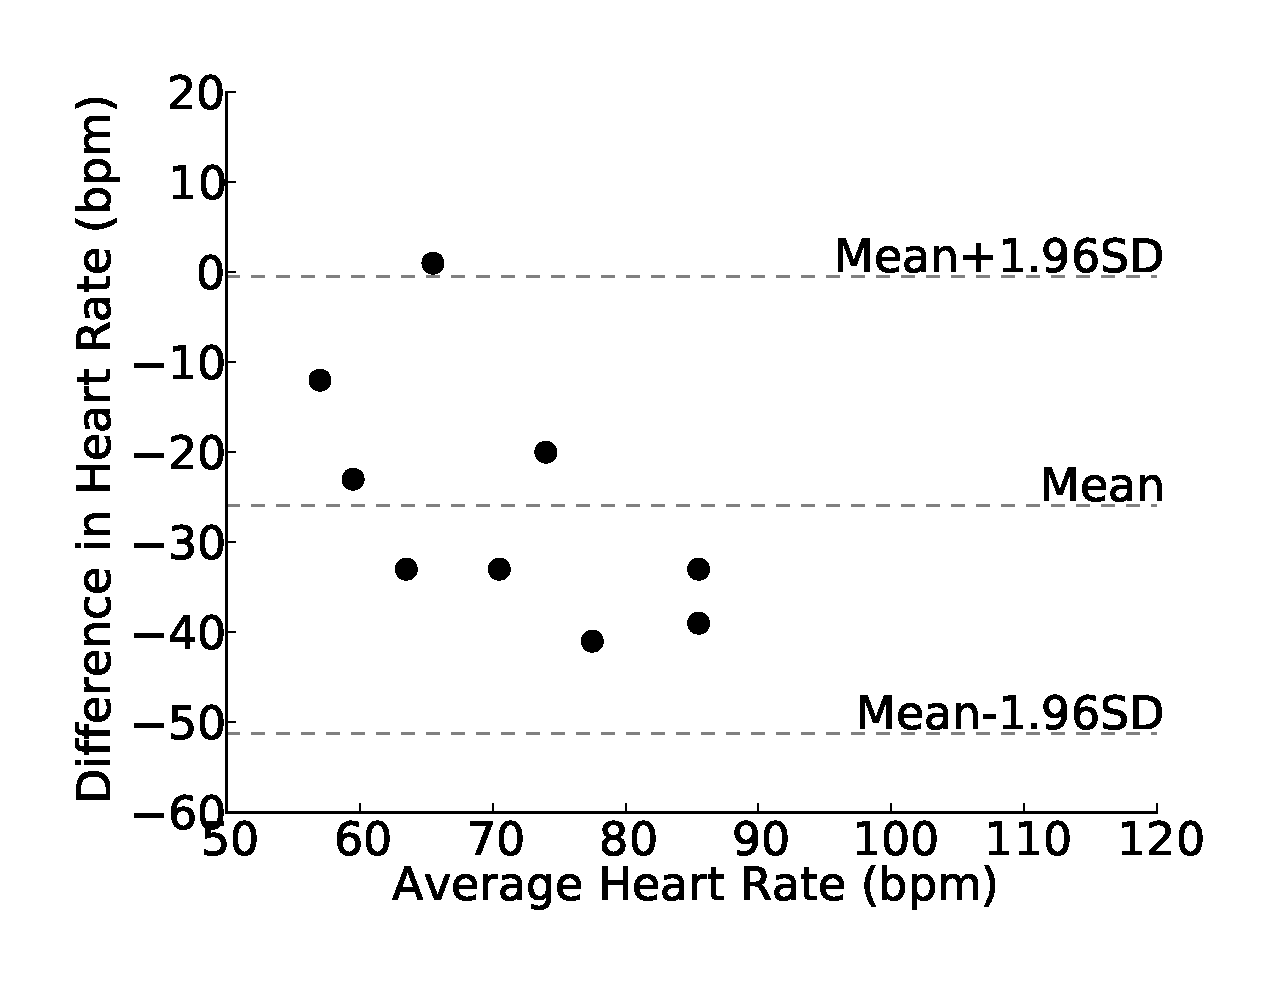
\includegraphics[width=\textwidth]{plots/pulse-after-exercise}
    \caption{Pulse and sphygmomanometer, after physical exercise.}
    \label{fig:plots:heart:pulse:exercise}
  \end{subfigure}
  ~
  \begin{subfigure}{0.5\textwidth}
    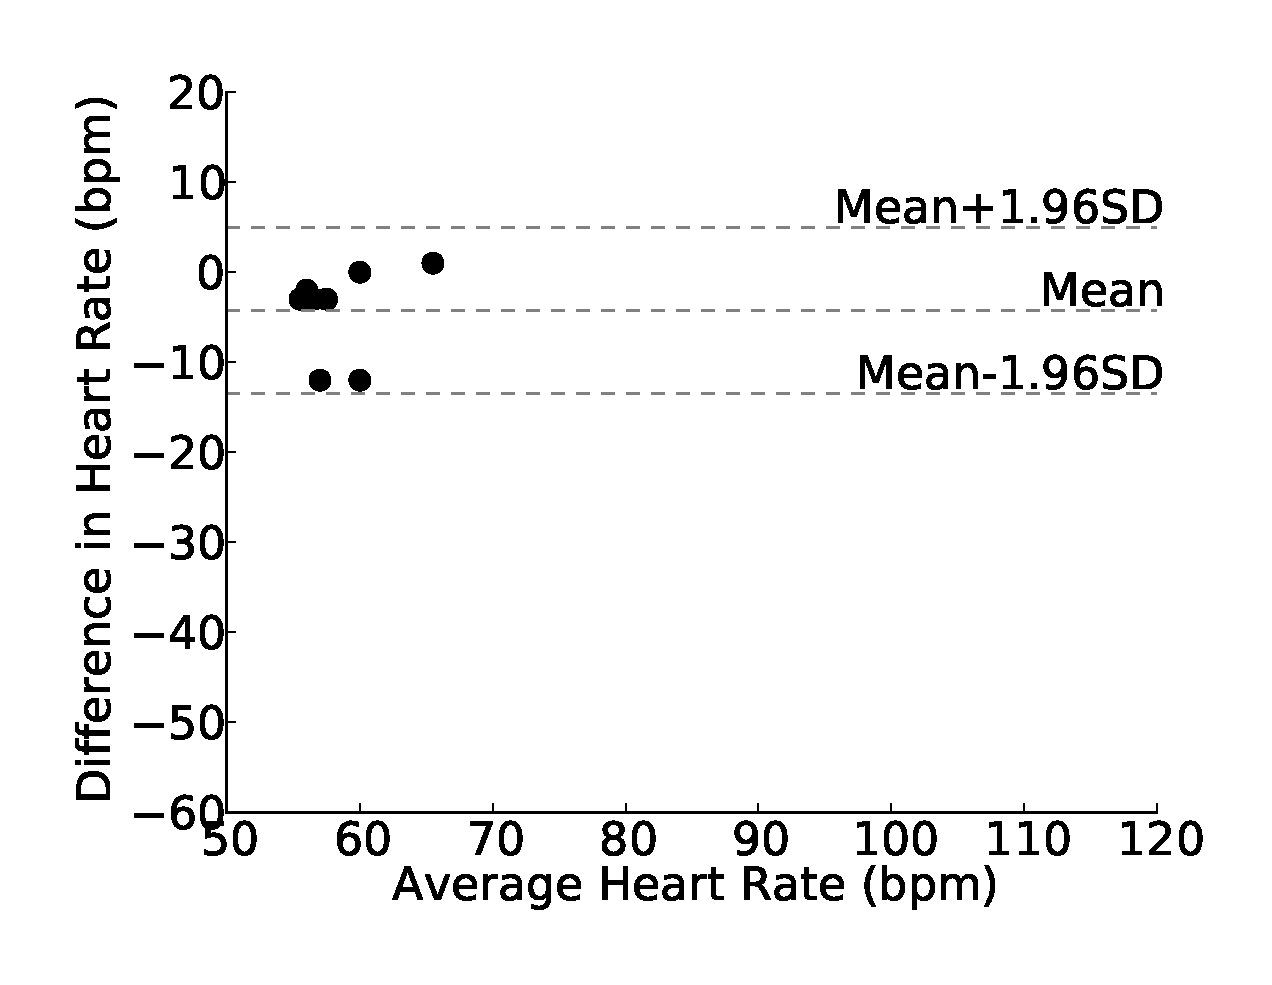
\includegraphics[width=\textwidth]{plots/pulse-lower-than-70-bpm}
    \caption{
      Pulse and sphygmomanometer, only measurements with an heart rate lower
      than 70 bpm according to the sphygmomanometer.
    }
    \label{fig:plots:heart:pulse:low}
  \end{subfigure}

  \caption{
    Bland-Altman plots demonstrating the agreement between the heart rate
    measurements obtained from a sphygmomanometer and an Android application:
    either Pulse, (a), (c), (d), which is the developed application,
    or the ViTrox application, (b).
  }
  \label{fig:plots:heart}
\end{figure}

\section{Chapter summary}

In this chapter, the performance optimizations of the algorithm and application
along with its metrics are presented. From a basic, real-time
implementation of the \evm{} method to an optimized version capable of
executing on an Android device at a reasonable rate of 15 frames per second
and a performance improvement of 22\%.

In addition, the heart rate estimations obtained using the
implemented Android application, Pulse, were compared to readings
from a sphygmomanometer and another Android application from
\emph{ViTrox Technologies}. Using Bland-Altman plots the best agreement
was between the Vitrox application and the sphygmomanometer, where the mean
bias was $1.33$ bpm with 95\% limits of agreement $-3.56$ to $6.22$ bpm.
Followed by the Pulse application and the sphygmomanometer, when the
beats per minute was lower than 70 according to the sphygmomanometer, with a
mean bias of $-4.25$ with 95\% limits of agreement $-13.43$ to $4.93$ bpm.
